%md->tex->template
\documentclass[12pt]{article}
\usepackage{CJKutf8}
\usepackage{amsmath}
\usepackage{geometry}
\usepackage{fancyhdr}
\usepackage{longtable,booktabs}
\usepackage{enumerate}
\usepackage{enumitem}
\usepackage{amsthm}
\usepackage{amssymb}
\usepackage{tikz}
\setlist[enumerate,1]{font=\bfseries}
\geometry{left=3.0cm,right=2.0cm,top=3.0cm,bottom=3.0cm}

\newenvironment{firstlayer}%
{\begin{list}{}{\renewcommand{\makelabel}[1]{\textbf{##1}.\hfil}
}}
{\end{list}}
\newenvironment{secondlayer}%
{\begin{list}{}{\renewcommand{\makelabel}[1]{(##1)\hfil}
}}
{\end{list}}

\renewcommand{\proofname}{\textbf{证明}}

\providecommand{\sol}{\textbf{解}.~}

\title{第 15 次作业}
\author{Log Creative}
\date{June 19, 2020}
\begin{document}

\begin{CJK}{UTF8}{gbsn}

\maketitle

\begin{firstlayer}
  \item[1]一棵树有$n_2$个结点的度为2,$n_3$个结点的度为3,$n_k$个结点的度为$k$。问有多少个度为1的节点。
  
  \sol 令有$n_1$个节点的度为1,没有度为0的节点(这是一棵树)。

节点数
$$n=\sum_{i=1}^kn_i$$

边数
$$n-1=\frac{\sum_{i=1}^k n_i i}{2}$$

解得:
$$n_1=2+\sum_{i=3}^k (i-2)n_i$$

\item[16]求图的最短树。

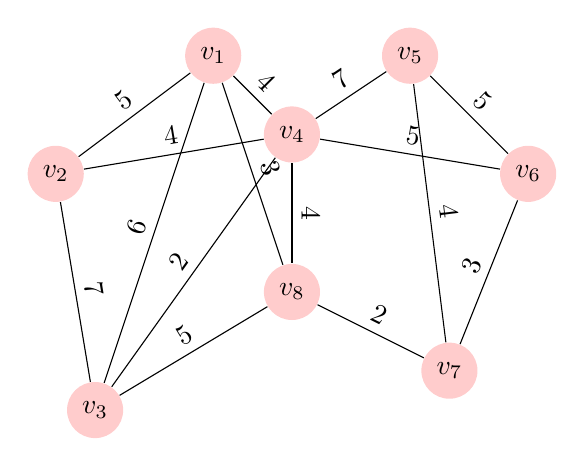
\begin{tikzpicture}

\node[circle,fill=red!20] (v1) at (-2,3.5) {$v_1$};
\node[circle,fill=red!20] (v2) at (-4,2) {$v_2$};
\node[circle,fill=red!20] (v3) at (-3.5,-1) {$v_3$};
\node[circle,fill=red!20] (v4) at (-1,2.5) {$v_4$};
\node[circle,fill=red!20] (v5) at (0.5,3.5) {$v_5$};
\node[circle,fill=red!20] (v6) at (2,2) {$v_6$};
\node[circle,fill=red!20] (v7) at (1,-0.5) {$v_7$};
\node[circle,fill=red!20] (v8) at (-1,0.5) {$v_8$};

\draw  (v1) edge node[above,sloped] {5}  (v2);
\draw  (v2) edge node[above,sloped] {7}  (v3);
\draw  (v3) edge node[above,sloped] {6} (v1);
\draw  (v2) edge node[above,sloped] {4}  (v4);
\draw  (v4) edge node[above,sloped] {2} (v3);
\draw  (v8) edge  node[above,sloped] {5} (v3);
\draw  (v4) edge  node[above,sloped] {4} (v8);
\draw  (v1) edge node[above,sloped] {3}  (v8);
\draw  (v4) edge node[above,sloped] {4} (v1);
\draw  (v5) edge node[above,sloped] {7} (v4);
\draw  (v6) edge node[above,sloped] {5} (v5);
\draw  (v4) edge node[above,sloped] {5} (v6);
\draw (v5) edge node[above,sloped] {4} (v7);
\draw  (v7) edge node[above,sloped] {3}(v6);
\draw  (v8) edge node[above,sloped] {2}(v7);
\end{tikzpicture}


\sol 使用Kruskal算法。

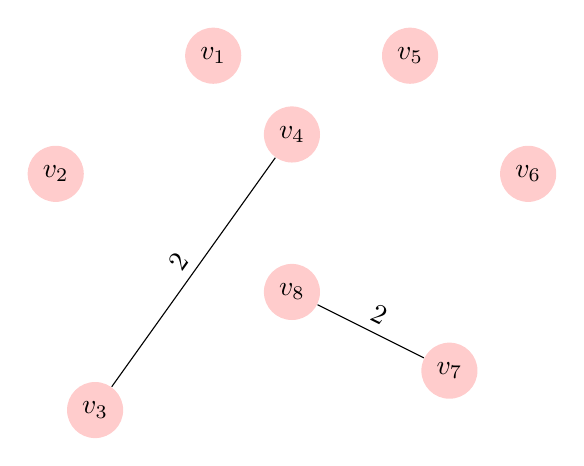
\begin{tikzpicture}

\node[circle,fill=red!20] (v1) at (-2,3.5) {$v_1$};
\node[circle,fill=red!20] (v2) at (-4,2) {$v_2$};
\node[circle,fill=red!20] (v3) at (-3.5,-1) {$v_3$};
\node[circle,fill=red!20] (v4) at (-1,2.5) {$v_4$};
\node[circle,fill=red!20] (v5) at (0.5,3.5) {$v_5$};
\node[circle,fill=red!20] (v6) at (2,2) {$v_6$};
\node[circle,fill=red!20] (v7) at (1,-0.5) {$v_7$};
\node[circle,fill=red!20] (v8) at (-1,0.5) {$v_8$};

%\draw  (v1) edge node[above,sloped] {5}  (v2);
%\draw  (v2) edge node[above,sloped] {7}  (v3);
%\draw  (v3) edge node[above,sloped] {6} (v1);
%\draw  (v2) edge node[above,sloped] {4}  (v4);
\draw  (v4) edge node[above,sloped] {2} (v3);
%\draw  (v8) edge  node[above,sloped] {5} (v3);
%\draw  (v4) edge  node[above,sloped] {4} (v8);
%\draw  (v1) edge node[above,sloped] {3}  (v8);
%\draw  (v4) edge node[above,sloped] {4} (v1);
%\draw  (v5) edge node[above,sloped] {7} (v4);
%\draw  (v6) edge node[above,sloped] {5} (v5);
%\draw  (v4) edge node[above,sloped] {5} (v6);
%\draw (v5) edge node[above,sloped] {4} (v7);
%\draw  (v7) edge node[above,sloped] {3}(v6);
\draw  (v8) edge node[above,sloped] {2}(v7);
\end{tikzpicture}
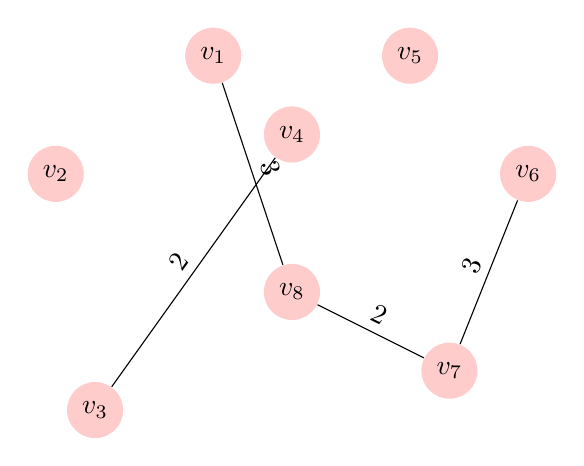
\begin{tikzpicture}

\node[circle,fill=red!20] (v1) at (-2,3.5) {$v_1$};
\node[circle,fill=red!20] (v2) at (-4,2) {$v_2$};
\node[circle,fill=red!20] (v3) at (-3.5,-1) {$v_3$};
\node[circle,fill=red!20] (v4) at (-1,2.5) {$v_4$};
\node[circle,fill=red!20] (v5) at (0.5,3.5) {$v_5$};
\node[circle,fill=red!20] (v6) at (2,2) {$v_6$};
\node[circle,fill=red!20] (v7) at (1,-0.5) {$v_7$};
\node[circle,fill=red!20] (v8) at (-1,0.5) {$v_8$};

%\draw  (v1) edge node[above,sloped] {5}  (v2);
%\draw  (v2) edge node[above,sloped] {7}  (v3);
%\draw  (v3) edge node[above,sloped] {6} (v1);
%\draw  (v2) edge node[above,sloped] {4}  (v4);
\draw  (v4) edge node[above,sloped] {2} (v3);
%\draw  (v8) edge  node[above,sloped] {5} (v3);
%\draw  (v4) edge  node[above,sloped] {4} (v8);
\draw  (v1) edge node[above,sloped] {3}  (v8);
%\draw  (v4) edge node[above,sloped] {4} (v1);
%\draw  (v5) edge node[above,sloped] {7} (v4);
%\draw  (v6) edge node[above,sloped] {5} (v5);
%\draw  (v4) edge node[above,sloped] {5} (v6);
%\draw (v5) edge node[above,sloped] {4} (v7);
\draw  (v7) edge node[above,sloped] {3}(v6);
\draw  (v8) edge node[above,sloped] {2}(v7);
\end{tikzpicture}

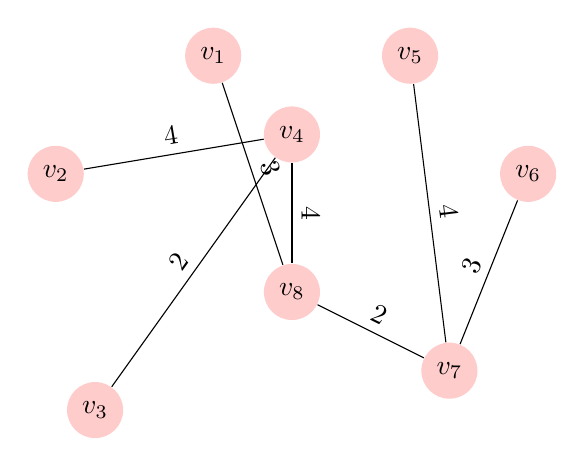
\begin{tikzpicture}

\node[circle,fill=red!20] (v1) at (-2,3.5) {$v_1$};
\node[circle,fill=red!20] (v2) at (-4,2) {$v_2$};
\node[circle,fill=red!20] (v3) at (-3.5,-1) {$v_3$};
\node[circle,fill=red!20] (v4) at (-1,2.5) {$v_4$};
\node[circle,fill=red!20] (v5) at (0.5,3.5) {$v_5$};
\node[circle,fill=red!20] (v6) at (2,2) {$v_6$};
\node[circle,fill=red!20] (v7) at (1,-0.5) {$v_7$};
\node[circle,fill=red!20] (v8) at (-1,0.5) {$v_8$};

%\draw  (v1) edge node[above,sloped] {5}  (v2);
%\draw  (v2) edge node[above,sloped] {7}  (v3);
%\draw  (v3) edge node[above,sloped] {6} (v1);
\draw  (v2) edge node[above,sloped] {4}  (v4);
\draw  (v4) edge node[above,sloped] {2} (v3);
%\draw  (v8) edge  node[above,sloped] {5} (v3);
\draw  (v4) edge  node[above,sloped] {4} (v8);
\draw  (v1) edge node[above,sloped] {3}  (v8);
%\draw  (v4) edge node[above,sloped] {4} (v1);
%\draw  (v5) edge node[above,sloped] {7} (v4);
%\draw  (v6) edge node[above,sloped] {5} (v5);
%\draw  (v4) edge node[above,sloped] {5} (v6);
\draw (v5) edge node[above,sloped] {4} (v7);
\draw  (v7) edge node[above,sloped] {3}(v6);
\draw  (v8) edge node[above,sloped] {2}(v7);
\end{tikzpicture}

\item[一 ] 设$G$是具有8个顶点的树,则$G$中增加多少条边才能把$G$变成完全图?

\sol 顶点数$$n=8+1=9$$

$$|E(K_n)|=\frac{n(n-1)}{2}=36$$

$$\Delta|E|=36-8=28$$

\item[二] 证明:设$G$是有$n$个结点的简单图,$n$是大于2的奇数.证明图$G$与它的补图$\bar{G}$中的奇数度结点个数相等。

\begin{proof}
  对于$G$中的一个奇数度节点,设其度数为$k$,因为是简单图,没有环,则$\bar{G}$中对应的节点度数为$n-k-1(n\geq 3)$,是奇数,则前后保持一致,则奇数度节点个数相等。
\end{proof}

\item[三] 设仅使用a ,b, c, d ,e, f这六种字符通信。使用a ,b, c, d ,e, f 的频率分别为4\%, 10\% ,16\%, 21\% ,23\% ,26\%。问:用Huffman算法求这六个字符的最佳前缀码。

\sol

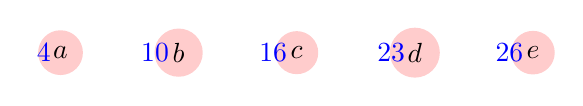
\begin{tikzpicture}
\node[circle,fill=red!20] (v1) at (-2,3.5) {$a$};
\node[circle,fill=red!20] (v2) at (-0.5,3.5) {$b$};
\node[circle,fill=red!20] (v3) at (1,3.5) {$c$};
\node[circle,fill=red!20] (v4) at (2.5,3.5) {$d$};
\node[circle,fill=red!20] (v5) at (4,3.5) {$e$};
\node[left,blue] at (v1) {4};
\node[left,blue] at (v2) {10};
\node[left,blue] at (v3) {16};
\node[left,blue] at (v4) {23};
\node[left,blue] at (v5) {26};
\end{tikzpicture}
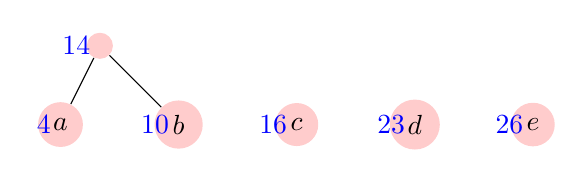
\begin{tikzpicture}
\node[circle,fill=red!20] (v1) at (-2,3.5) {$a$};
\node[circle,fill=red!20] (v2) at (-0.5,3.5) {$b$};
\node[circle,fill=red!20] (v3) at (1,3.5) {$c$};
\node[circle,fill=red!20] (v4) at (2.5,3.5) {$d$};
\node[circle,fill=red!20] (v5) at (4,3.5) {$e$};
\node[circle,fill=red!20] (v6) at (-1.5,4.5) {};
\node[left,blue] at (v1) {4};
\node[left,blue] at (v2) {10};
\node[left,blue] at (v3) {16};
\node[left,blue] at (v4) {23};
\node[left,blue] at (v5) {26};
\node[left,blue] at (v6) {14};
\draw  (v6) edge (v1);
\draw  (v6) edge (v2);
\end{tikzpicture}

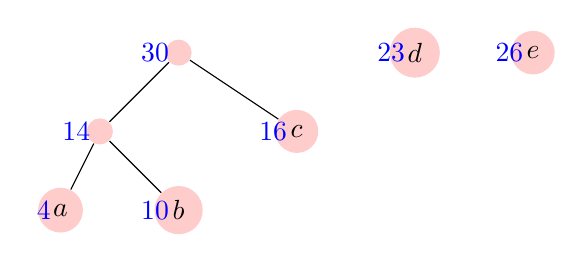
\begin{tikzpicture}
\node[circle,fill=red!20] (v1) at (-2,3.5) {$a$};
\node[circle,fill=red!20] (v2) at (-0.5,3.5) {$b$};
\node[circle,fill=red!20] (v3) at (1,4.5) {$c$};
\node[circle,fill=red!20] (v4) at (2.5,5.5) {$d$};
\node[circle,fill=red!20] (v5) at (4,5.5) {$e$};
\node[circle,fill=red!20] (v6) at (-1.5,4.5) {};
\node[circle,fill=red!20] (v7) at (-0.5,5.5) {};
\node[left,blue] at (v1) {4};
\node[left,blue] at (v2) {10};
\node[left,blue] at (v3) {16};
\node[left,blue] at (v4) {23};
\node[left,blue] at (v5) {26};
\node[left,blue] at (v6) {14};
\node[left,blue] at (v7) {30};
\draw  (v6) edge (v1);
\draw  (v6) edge (v2);
\draw  (v7) edge (v6);
\draw  (v7) edge (v3);
\end{tikzpicture}
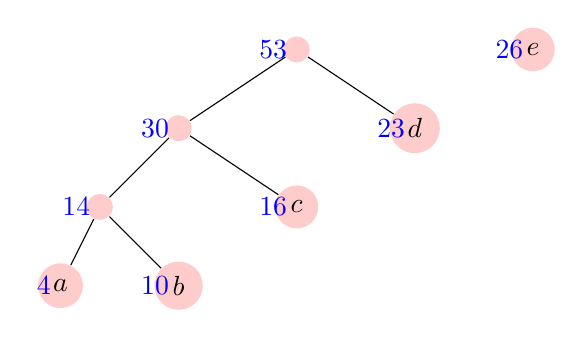
\begin{tikzpicture}
\node[circle,fill=red!20] (v1) at (-2,3.5) {$a$};
\node[circle,fill=red!20] (v2) at (-0.5,3.5) {$b$};
\node[circle,fill=red!20] (v3) at (1,4.5) {$c$};
\node[circle,fill=red!20] (v4) at (2.5,5.5) {$d$};
\node[circle,fill=red!20] (v5) at (4,6.5) {$e$};
\node[circle,fill=red!20] (v6) at (-1.5,4.5) {};
\node[circle,fill=red!20] (v7) at (-0.5,5.5) {};
\node[circle,fill=red!20] (v8) at (1,6.5) {};
\node[left,blue] at (v1) {4};
\node[left,blue] at (v2) {10};
\node[left,blue] at (v3) {16};
\node[left,blue] at (v4) {23};
\node[left,blue] at (v5) {26};
\node[left,blue] at (v6) {14};
\node[left,blue] at (v7) {30};
\node[left,blue] at (v8) {53};
\draw  (v6) edge (v1);
\draw  (v6) edge (v2);
\draw  (v7) edge (v6);
\draw  (v7) edge (v3);
\draw  (v8) edge (v7);
\draw  (v8) edge (v4);
\end{tikzpicture}

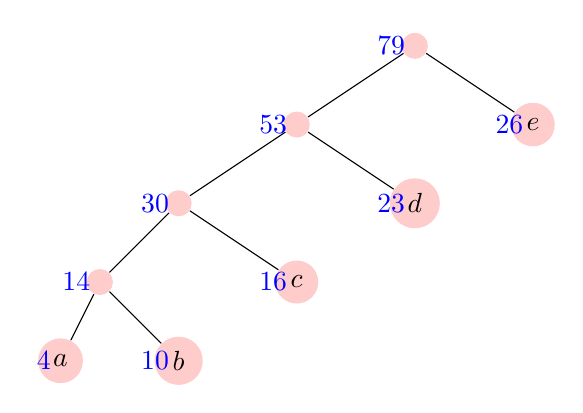
\begin{tikzpicture}
\node[circle,fill=red!20] (v1) at (-2,3.5) {$a$};
\node[circle,fill=red!20] (v2) at (-0.5,3.5) {$b$};
\node[circle,fill=red!20] (v3) at (1,4.5) {$c$};
\node[circle,fill=red!20] (v4) at (2.5,5.5) {$d$};
\node[circle,fill=red!20] (v5) at (4,6.5) {$e$};
\node[circle,fill=red!20] (v6) at (-1.5,4.5) {};
\node[circle,fill=red!20] (v7) at (-0.5,5.5) {};
\node[circle,fill=red!20] (v8) at (1,6.5) {};
\node[circle,fill=red!20] (v9) at (2.5,7.5) {};
\node[left,blue] at (v1) {4};
\node[left,blue] at (v2) {10};
\node[left,blue] at (v3) {16};
\node[left,blue] at (v4) {23};
\node[left,blue] at (v5) {26};
\node[left,blue] at (v6) {14};
\node[left,blue] at (v7) {30};
\node[left,blue] at (v8) {53};
\node[left,blue] at (v9) {79};
\draw  (v6) edge (v1);
\draw  (v6) edge (v2);
\draw  (v7) edge (v6);
\draw  (v7) edge (v3);
\draw  (v8) edge (v7);
\draw  (v8) edge (v4);
\draw  (v9) edge (v8);
\draw  (v9) edge (v5);
\end{tikzpicture}

最佳前缀码:
\begin{align*}
  a&=0000\\
b&=0001\\
c&=001\\
d&=01\\
e&=1
\end{align*}


\end{firstlayer}


\end{CJK}

\end{document}

